In the following sequence diagrams, we describe exactly the interactions between the key actors our system. It is important to note that most of the interaction between the user (or league manager or site administrator) and system is facilitated by the browser. The user, through filling forms and button clicks, instructs the browser which requests to make to the system. In turn, the system communicates with the database to request the desired data, takes any required actions, and delivers the data to the browser for presentation to the user.

\begin{figure}
\centering
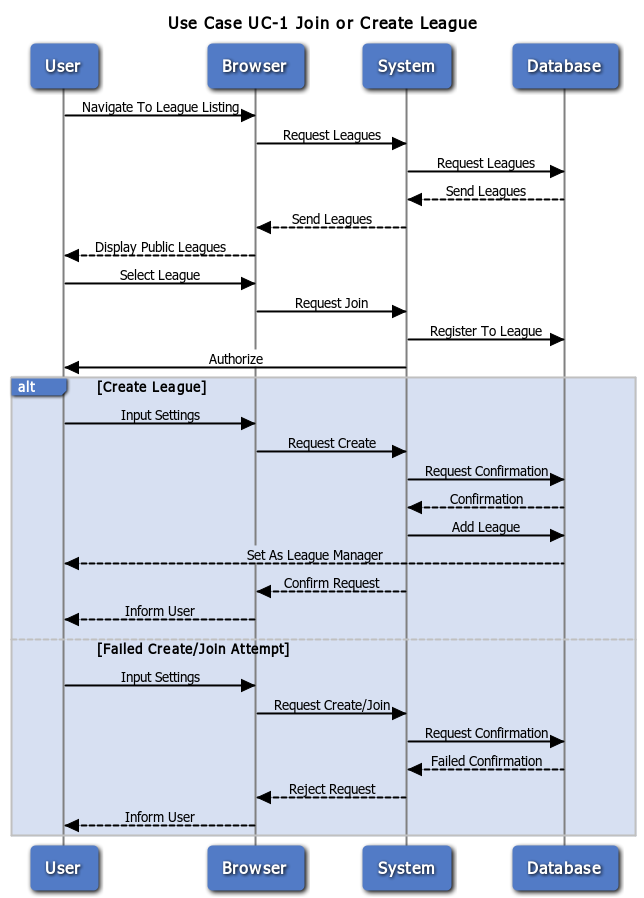
\includegraphics[width=5.5in]{./Diagrams/SystemSequenceDiagrams/uc1.png}
\caption{See UC-1 on page \pageref{UC-1}. When the user navigates to the league listing page, they invoke this use case. The user initiates a request to view all the public leagues and the system retrieves them from the database. Then, they are presented to the user who is given the option to join any valid league.}
\end{figure}

\begin{figure}
\centering
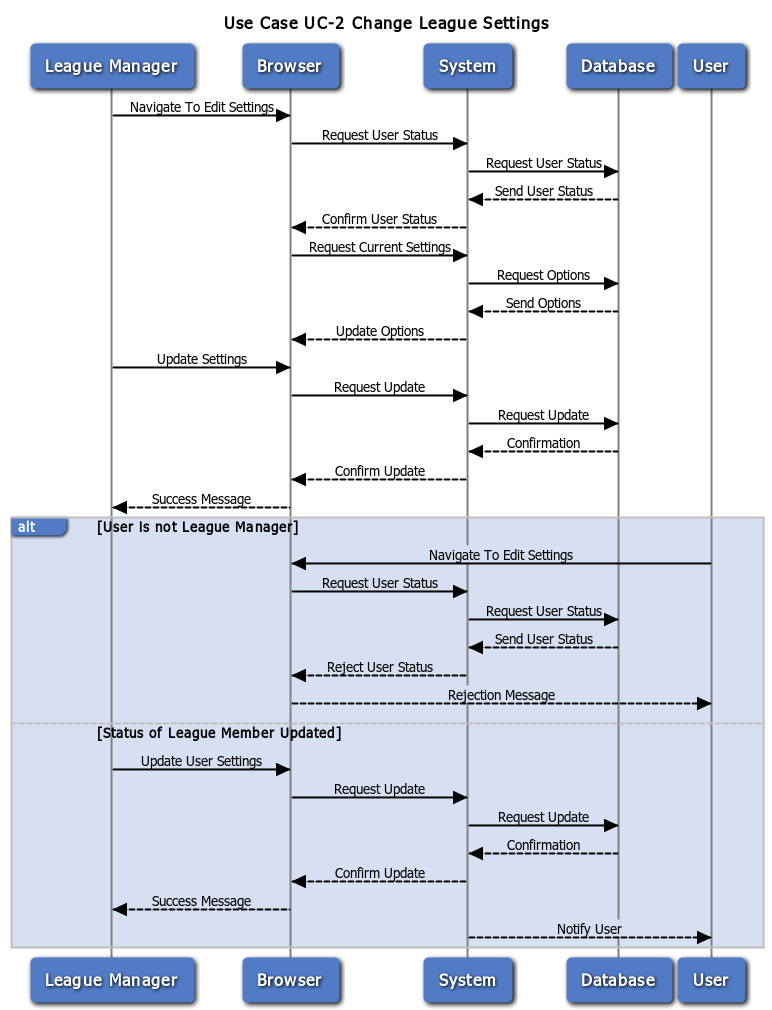
\includegraphics[width=5.5in]{./Diagrams/SystemSequenceDiagrams/uc2.png}
\caption{See UC-2 on page \pageref{UC-2}. This is sequence of events that occur when a league manager alters the league settings. The system fetches the current settings from the database and returns them to the browser. It also ensures that the user attempting this change is a league manager. Then, the user can initiate a request to change the settings which will be enacted out by the system. If the league manager changes the status of a user within the league, the system notifies that user.}
\end{figure}

\begin{figure}
\centering
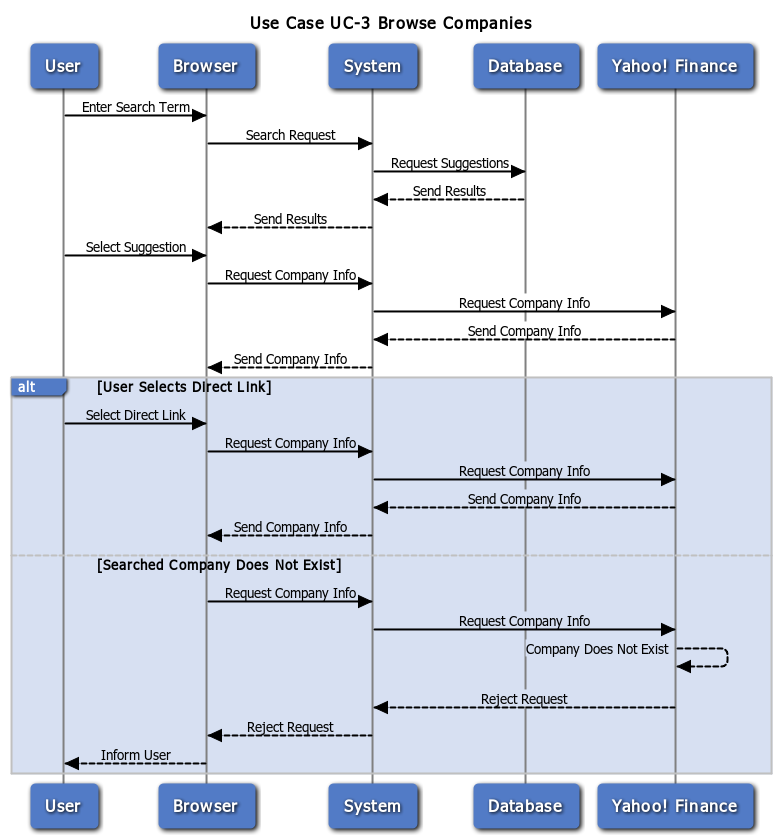
\includegraphics[width=5.5in]{./Diagrams/SystemSequenceDiagrams/uc3.png}
\caption{See UC-3 on page \pageref{UC-3}. When the user desires to research companies, this is the sequence that follows. The user is able to search and browse for companies. They can also get to a company's page through a direct link. Yahoo! Finance responds to requests and delivers data to our system which is then transferred to the browser and fills out a company profile.}
\end{figure}

\begin{figure}
\centering
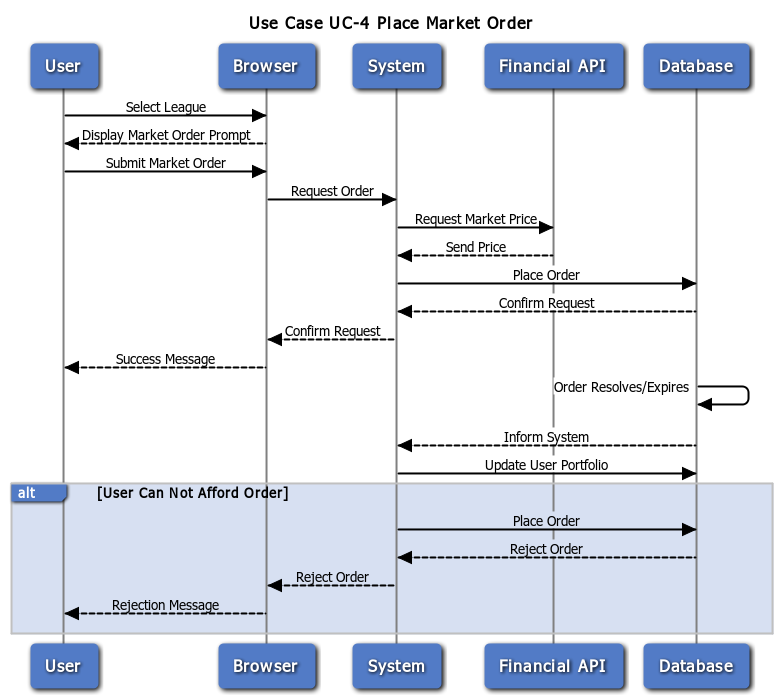
\includegraphics[width=5.5in]{./Diagrams/SystemSequenceDiagrams/uc4.png}
\caption{See for UC-4 on page \pageref{UC-4}. This sequence encompasses the bread and butter of our application--market orders. The user selects a league in which to place an order, fills out a prompt in the browser which then submits the request to the system. The system inserts the order into the database and enqueues it (the queuing system will be elaborated upon in a later section). Once the order resolves or expires, the database notifies the system and the user's portfolio is updated accordingly.}
\end{figure}

\begin{figure}
\centering
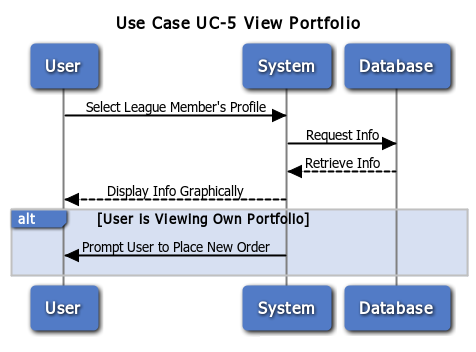
\includegraphics[width=5.5in]{./Diagrams/SystemSequenceDiagrams/uc5.png}
\caption{See UC-5 on page \pageref{UC-5}. This use case is relatively straightforward. The user browses to a league member's portfolio, and the browser submits a request to the database for that portfolio's inormation.}
\end{figure}

\begin{figure}
\centering
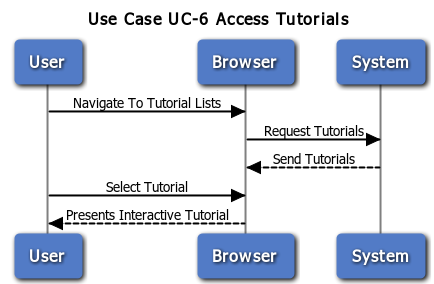
\includegraphics[width=5.5in]{./Diagrams/SystemSequenceDiagrams/uc6.png}
\caption{See UC-6 on page \pageref{UC-6}. Another simple use case. The user simply navigates to the tutorial page, which is populated by the system.}
\end{figure}

\begin{figure}
\centering
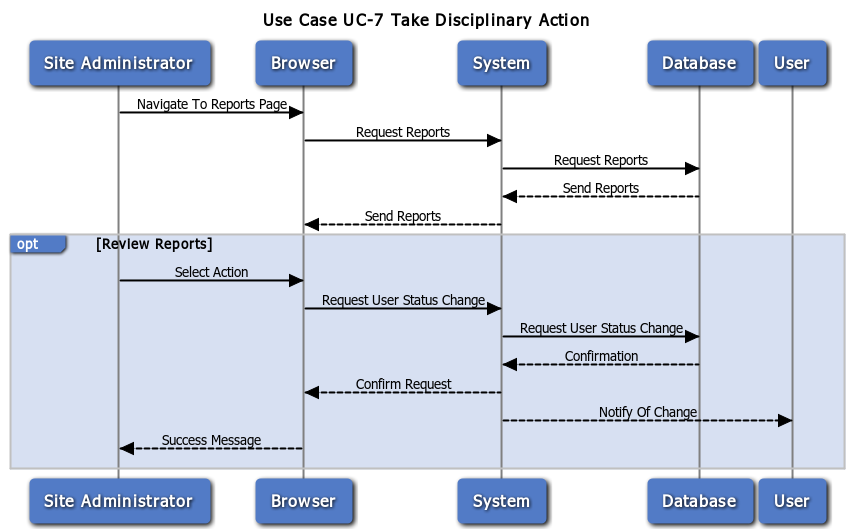
\includegraphics[width=5.5in]{./Diagrams/SystemSequenceDiagrams/uc7.png}
\caption{See UC-7 on page \pageref{UC-7}. When a site administrator navigates to observe any outstanding abuse reports, this flow of events is initiated. The database delivers all outstanding reports to the system which then populates them in the browser. If the administrator decides to take an action, the status change is reflected in the database, and the system notifies the user of whatever action was taken against them.}
\end{figure}
